%El principal objetivo del presente Trabajo Integrador es el de proveer una comunicación USB para desarrollos basados en FPGA. Por esto mismo, es fundamental sintetizar un circuito en el FPGA que sirva de nexo entre el desarrollo y la placa de interfaz.\\

%Es por esto que se utilizó 
%Para la implementación de la comunicación de un desarrollo determinado, se requiere un nexo entre la síntesis del circuito y la memoria del controlador USB. Este vínculo se lleva a cabo mediante una pequeña MEA que ejecuta las señales de lectura y escritura. Esta MEA se desarrolla en lenguaje VHDL.\\
Para trasmitir información en un sistema de comunicación, los componentes que intervienen siguen un protocolo determinado. Así, no solo se facilita el envío y la recepción del mensaje, sino también que determina a cada dispositivo los procedimiento que debe efectuar. Por este motivo, una vez definido que se utiliza una interfaz intermedia entre la PC y un FPGA (Capítulo~\ref{cap:int}), y que dicha interfaz es el circuito integrado EZ-USB FX2LP de Cypress (Capítulo~\ref{cap:cy}), se determina cuál es el protocolo a través del cuál se comunica cada uno de los dispositivos y se puede configurar un FPGA para que reciba y envíe datos a la interfaz.

En base a los materiales disponibles, se evaluaron tres placas de desarrollo diferentes, todas con FPGA diseñadas y comercializadas por la empresa Xilinx Inc. La placa Spartan-3E Starter, comercializada por Digilent, tiene como dispositivo central un FPGA Spartan 3. Además, posee una gran cantidad de periféricos, entre los que se destacan su pantalla LCD, los \SI{18}{\mega\byte} de memoria flash sumados a \SI{64}{\mega\byte} de SDRAM y transceptores varios, tales como Ethernet, PS/2 para teclados y JTAG para programación y depuración.

Por su parte, la placa Nexys 3, tiene como núcleo un FPGA Spartan 6. Este dispositivo brinda mayor cantidad de bloques lógicos programables que la versión Spartan 3, debido a que posee transistores más pequeños gracias a un proceso de fabricación CMOS más moderno. La miniaturización de los transistores, a su vez, otorga la posibilidad de una mayor velocidad de operación. La placa Nexis 3 también posee una gran gama de periféricos tales como pulsadores, interruptores, displays led de 7 segmentos, diferentes tipos de memorias, CODEC para comunicarse por Ethernet 10/100 o USB 2.0 de máxima velocidad (\SI{12}{\mega\bit\per\second}).

A diferencia de las anteriores, la placa de desarrollo Mojo v3 comercializada por la empresa Alchitry, es una placa de prototipado rápido. Esto quiere decir que en lugar de poseer una gran cantidad y variedaad de periféricos, se dota a la placa de una gran cantidad de puertos para que el usuario pueda colocar los perifércios que desea. Al igual que la Nexys 3, cuenta con un FPGA Spartan 6 de Xilinx. Dispone de 84 puertos digitales configurables como entrada y/o salida, 8 entradas analógicas, 8 LED's de propósito general, un botón de tipo pulsador. La principal ventaja de esta placa de desarrollo es que posee un costo notablemente inferior a las anteriores debido en gran medida a la ausencia de periféricos que, dependiendo la aplicación, pueden ser innecesarios.

Se elige para el desarrollo que se presenta en este trabajo la placa de desarrollo Mojo v3 debido a que posee un FPGA superior a la placa Spartan 3E Starter, brindando la posibilidad de elaborar sistemas más complejos y veloces. A su vez, es más económica que la placa Nexys 3, que posee un FPGA de similares características. En otras palabras la Mojo se selecciona por su bajo costo, versatilidad y por que está dotada por un Spartan 6 de Xilinx, que es un FPGA con una buena relación entre recursos, rendimiento, velocidad y precio. La menor disponibilidad de periféricos de la placa Mojo v3 con respecto a las otras placas de desarrollo, no es un inconveniente porque el kit CY3684 de Cypress incorpora los dispositivos necesarios para los fines de este trabajo.
%utilizado para el desarrollo de la interfaz. Además de esto, posee un FPGA superior a la placa Spartan 3E Starter, por lo que brinda la posibilidad de elaborar sistemas más complejos y veloces. 
%Existe en el mercado una amplia variedad de FPGA, como así también de placas de desarrollo que permiten desarrollar sistemas con este tipo de ciruitos integrados. El equipo de trabajo posee una placa de desarrollo Spartan-3E Starter, la cual posee como FPGA un Spartan-3 de Xilinx. Sin embargo esta placa se encuentra obsoleta, por cuanto es dificil de conseguir soporte y no es aconsejable realizar un diseño nuevo con este tipo de placas. 
%
%Por su parte el 

%Se elige para este trabajo, la placa de desarrollo MOJO v3 desarrollada por la empresa Embedded Micro. Esta placa, la cual se observa en la Figura \ref{mojo}, posee un FPGA Spartan-6 de Xilinx. El FPGA brinda la posibilidad de elaborar sistemas digitales complejos de alta velocidad y permite, al desarrollador de sensores y sistemas de adquisición de datos, la síntesis de circuitos que resuelvan problemas en la medida de los requerimientos. Dispone también de 84 puertos digitales configurables como entrada y/o salida, 8 entradas analógicas, 8 LED's de propósito general, un botón de tipo pulsador.

La Mojo v3, la cual se observa en la Figura \ref{mojo}, es una placa de desarrollo muy económica para prototipado, es decir, la fabricación de modelos funcionales. Para ello los puertos se disponen en un arreglo de pines a través de los cuales es posible acoplar el dispositivo que sea necesario. Se dispone en el mercado de otros circuitos impresos que se conectan a los pines y contienen un grupo de periféricos para propósito general. Estos circuitos impresos, se denominan \textit{shields}\footnote{ \textit{Shield} es una palabra del habla inglesa que en español significa escudo o armadura. Su pronunciación suena como \textit{shild}}. El usuario también puede diseñar sus propios \textit{shields} o conectar las entradas y salidas de otros dispositivo mediante cables, conformando así una placa de desarrollo a la medida de las necesidades de cada proyecto.%\\

\begin{figure}[ht]
	\centering
	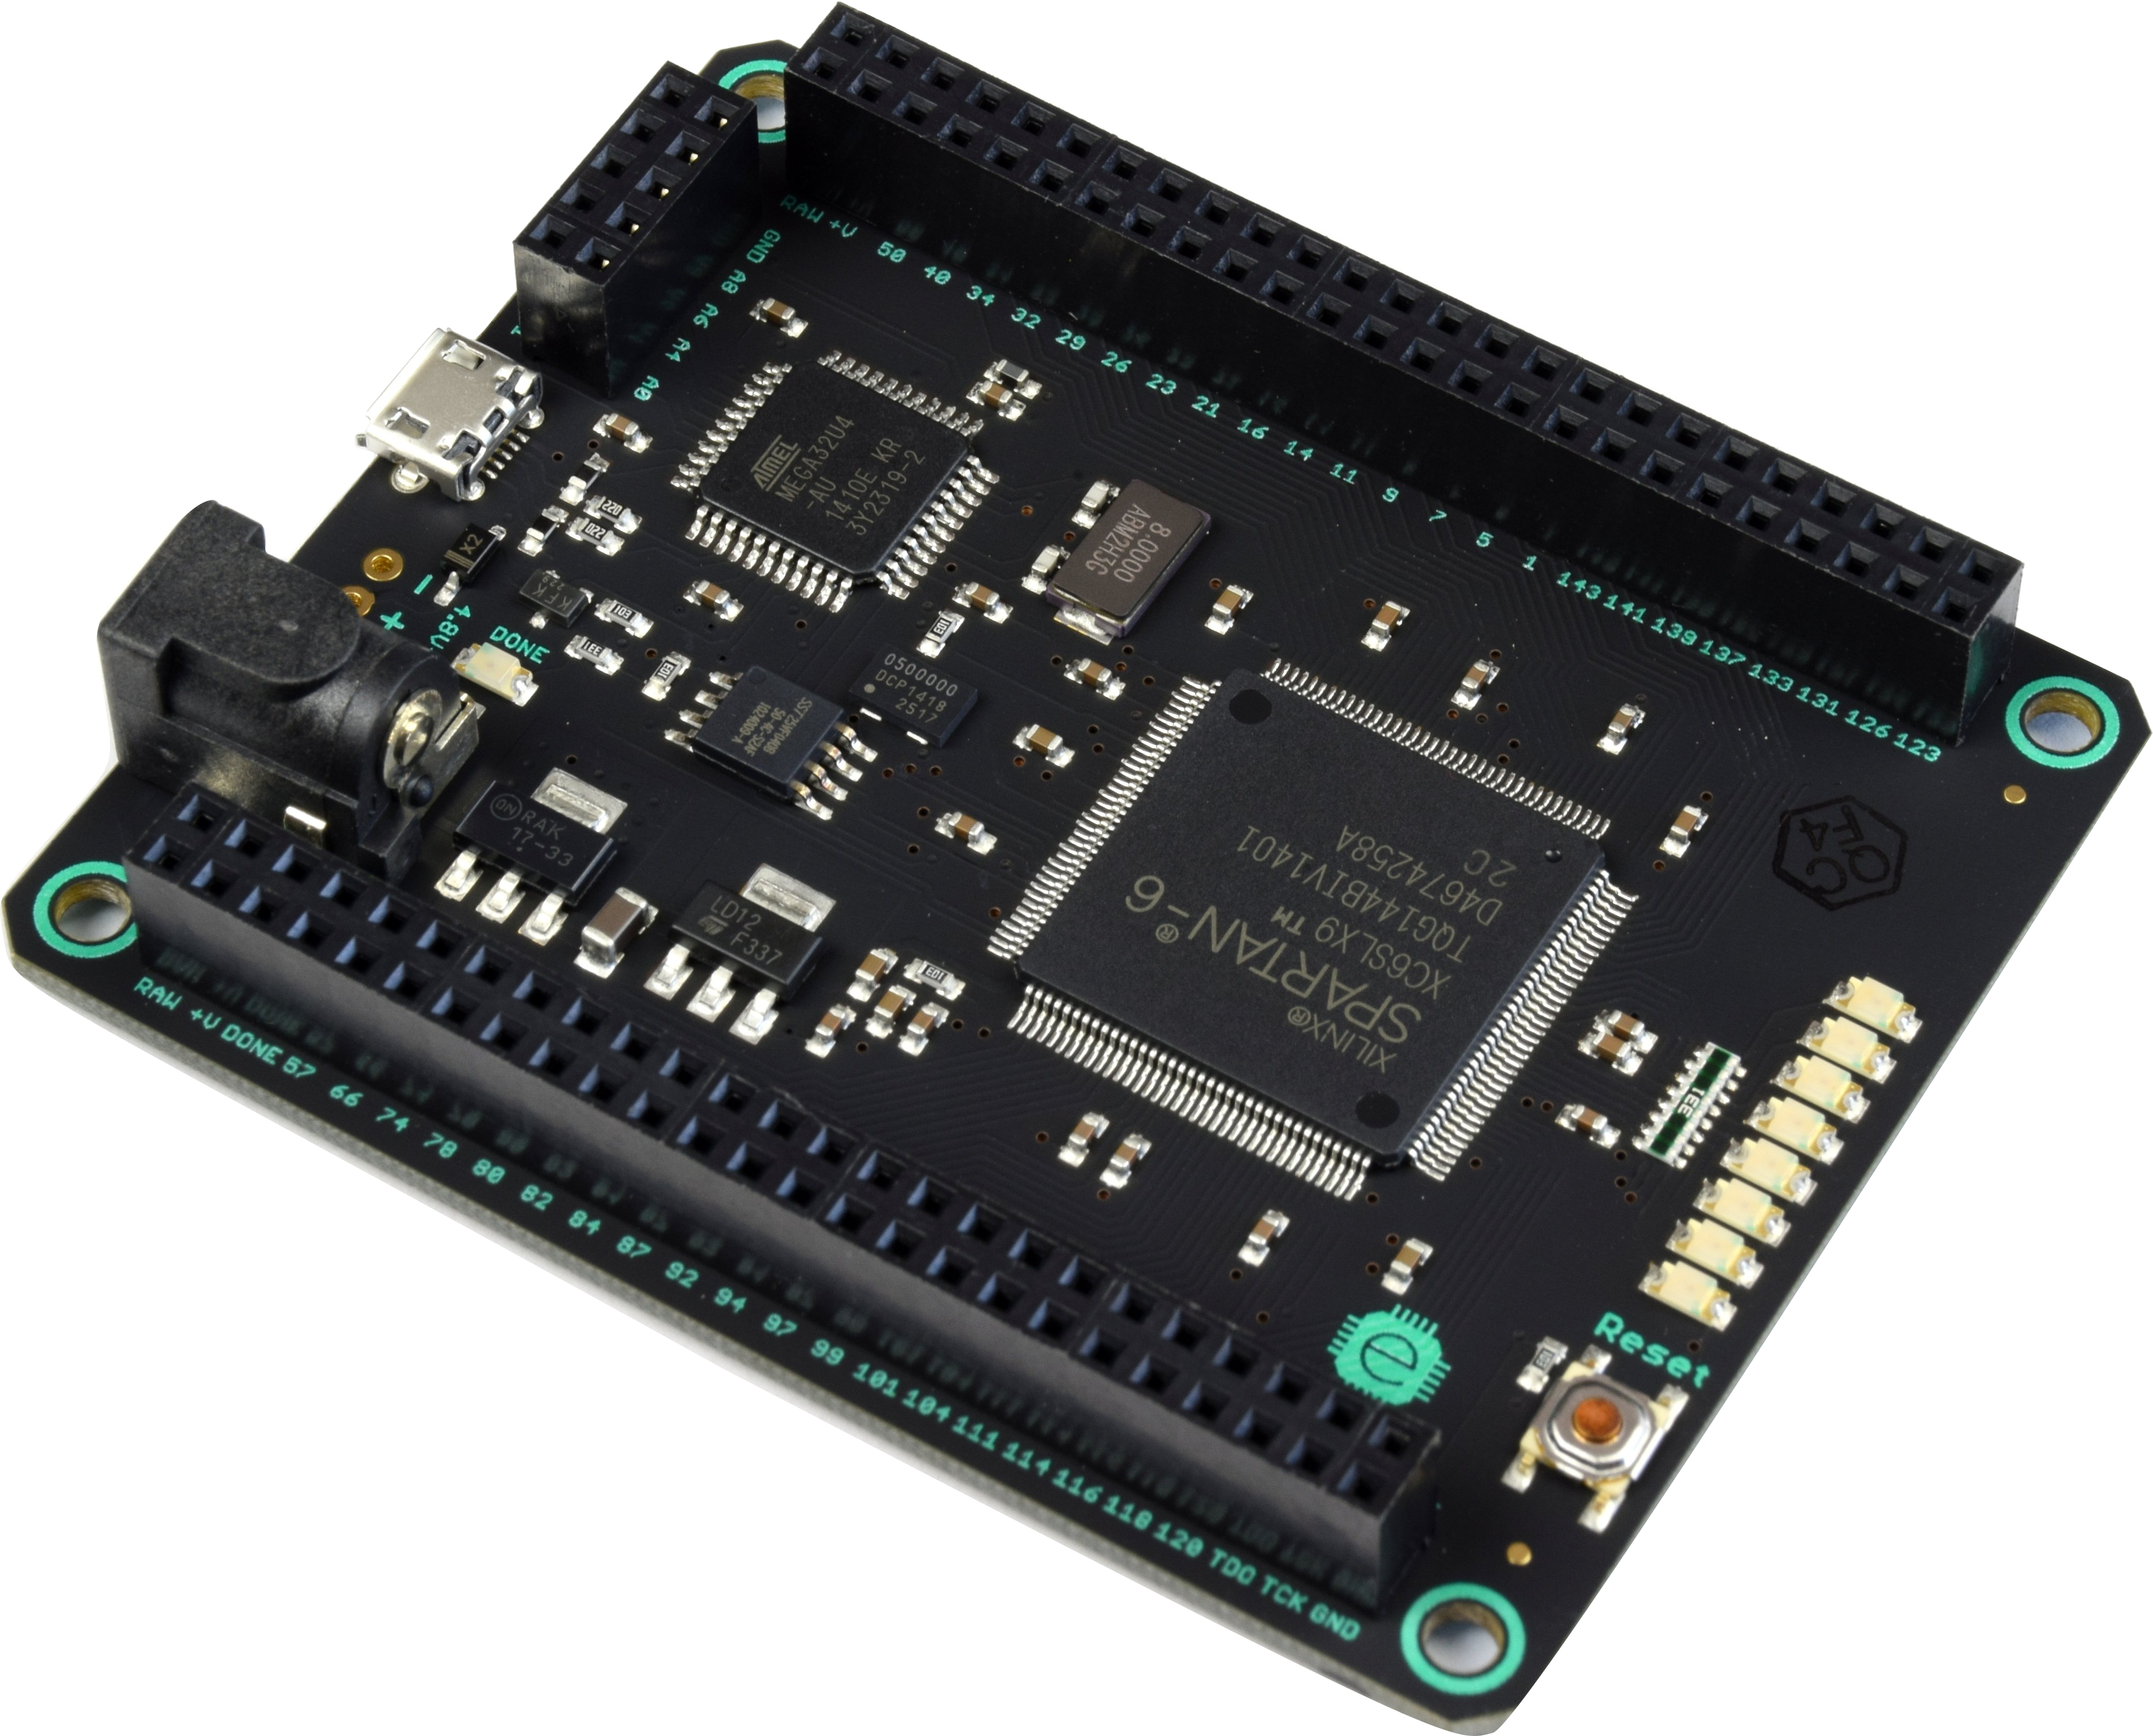
\includegraphics[width = 0.4\textwidth]{mojov3}
	\caption{Placa de prototipado rápido MOJO v3, diseñada por Embedded Micro}
	\label{mojo}
\end{figure}

Además de los \textit{shields}, los diseñadores pensaron en que no sea necesario ninguna herramienta extra a la hora de programar la FPGA. Para ello, dotaron al sistema de un $\mu$C ATmega32U4 diseñado por la empresa Atmel con un programa de tipo bootloader, que se encarga de transferir la configuración del FPGA (cargada desde una memoria flash incorporada, o trasmitida por el usuario desde una PC), a través de un transceptor USB que contiene el $\mu$C. Luego, el controlador es colocado en modo esclavo y se configura de forma tal que dota al sistema de una comunicación entre la FPGA y una PC, vía USB. Las entradas analógicas que posee esta placa de desarrollo también son leídas a través del $\mu$C ATmega32U4, luego de que el FPGA es programado.%\\%Luego, entra en modo esclavo, lo que permite al usuario, a posterior poder usar para debug el sistema USB que posee el microcontrolador.\\

%Una vez llegado a este punto, el lector podría preguntar con toda razón ¿por qué es necesario realizar un sistema de comunicación USB extra, si ya cuenta con un microcontrolador que se encarga de dicho asunto? La respuesta se basa en el ancho de banda del sistema de comunicación que dispone la placa.
Es importante aclarar que si bien el sistema posee alguna forma de comunicación USB utilizando el $\mu$C ATmega32U4 como interfaz, este enlace posee un menor ancho de banda que el sistema desarrollado en el presente trabajo. Esto se debe a que la línea de controladores ATmega incorpora puertos USB 2.0 de máxima velocidad (\SI{12}{\mega\bit\per\second})~\cite{Atmel2016}. Además, la comunicación entre ambos chips se realiza vía SPI (\textit{Serial Peripherical Interface}, o en español Interfaz Serie de Periféricos), con una tasa de transferencia máxima de \SI{8}{\mega\bit\per\second}~\cite{Atmel2016}, ya sea para transmitir por el puerto USB como para comunicar las entradas analógicas digitalizadas, ofreciendo una velocidad de salida que puede resultar insuficiente a los fines de este trabajo. Se pretende dotar al sistema del mayor ancho de banda posible, utilizando la capacidad de USB 2.0 de alta velocidad, de hasta \SI{480}{\mega\bit\per\second}.